\documentclass[english]{beamer}
\useoutertheme{RJTcustom}

\begin{document}

\begin{frame}{Lecture 02W Plan}
  \textbf{Administrative}
  \begin{itemize}
    \item No class or lab on Monday
  \end{itemize}
  \textbf{Material}
  \begin{itemize}
    \item Newton's Second Law
    \item The weight force
    \item The dry friction force
    \item The fluid friction (drag) force
  \end{itemize}
\end{frame}

\begin{frame}{Newton's Second Law}
  Newton's 1st Law says \textbf{no net force = no acceleration}. What if there \emph{is} a net force?
\end{frame}

\begin{frame}{Newton's Second Law: two parts}
  \begin{figure}[!tbp]
    \begin{minipage}[b]{0.4\textwidth}
      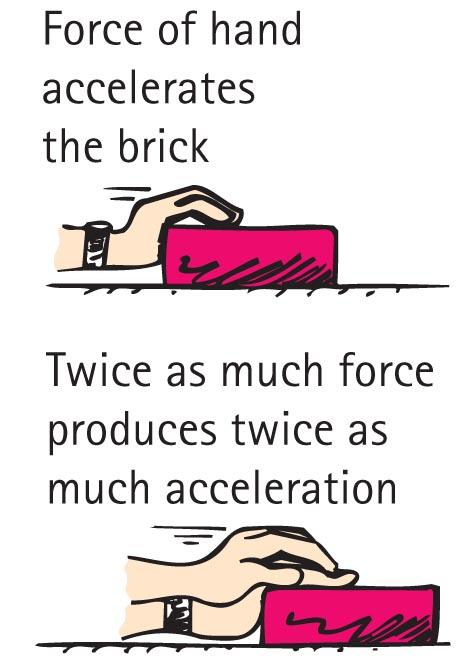
\includegraphics[height=0.6\textheight]{./04_02_Figure_cropped.jpg}
    \end{minipage}
    \begin{minipage}[b]{0.4\textwidth}
      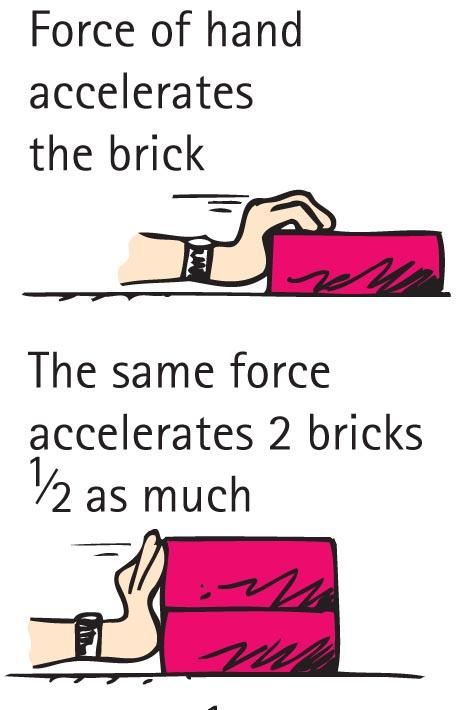
\includegraphics[height=0.6\textheight]{./04_11_Figure_cropped.jpg}
    \end{minipage}
  \end{figure}
  \begin{itemize}
    \item Acceleration increases as net force increases: $a \propto \sigma F$
    \item Acceleration increases as mass decreases: $a \propto \frac{1}{m}$
  \end{itemize}
\end{frame}

\begin{frame}{Newton's Second Law}
  \begin{itemize}
    \item Acceleration increases as net force increases: $a \propto \sigma F$
    \item Acceleration increases as mass decreases: $a \propto \frac{1}{m}$
  \end{itemize}
  We can combine these two observations:
  \begin{center}
    $\text{acceleration} = \frac{\text{net force}}{\text{mass}}$\\
  \end{center}
\end{frame}

\begin{frame}{Newton's Second Law}
  Check your understanding: 
  \begin{itemize}
    \item Relate this to the definition of acceleration: $\mathbf{a} \equiv \frac{\Delta \mathbf{v}}{\Delta t}$?
    \item What are the units of acceleration?
    \item What are the units of mass? 
    \item What are the units of force? (Can we express this unit in two ways?)
  \end{itemize}
\end{frame}

\begin{frame}{The weight force}
  \begin{itemize}
    \item Free-fall acceleration for any mass is $g$. What is the weight force?
    \item Combine $a=g$ and $a=\frac{F}{m}$ to get $F_{\text{weight}}=m\,g$.
    \item Note: $g$ is different on different planets.
    \item It is \emph{not} different in orbit!
    \item (We will discuss the \emph{universal} gravitational force in a few weeks.)
  \end{itemize}
\end{frame}

\begin{frame}{The weight force}
  Check your understanding:
  \begin{itemize}
    \item The acceleration of a piano and a pin in free-fall are the same. Does that mean that gravity pulls on them with the same force?
  \end{itemize}
  \visible<2->{
    \begin{figure}[h]
      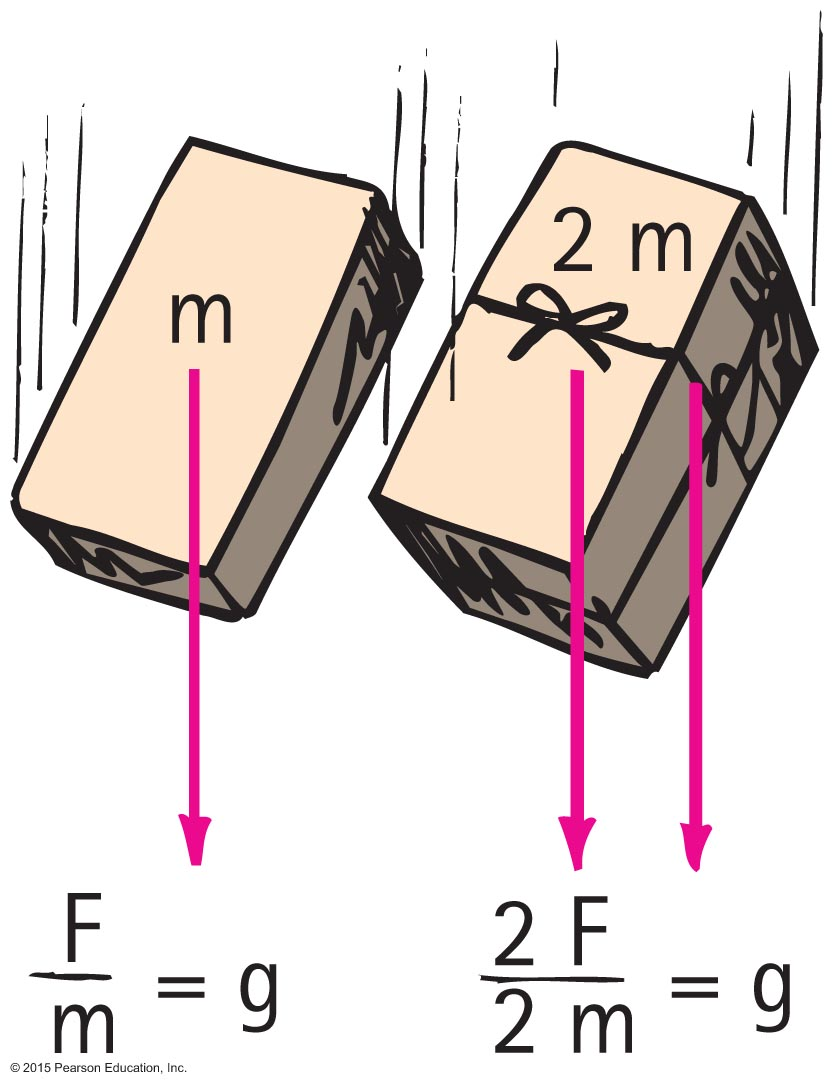
\includegraphics[width=4cm]{./04_12_Figure.jpg}
    \end{figure}
  }
\end{frame}

\begin{frame}{The dry friction force}

\end{frame}

\begin{frame}{The fluid friction (drag) force}

\end{frame}

\end{document}
